\documentclass[a4paper,10pt]{beamer}
\usepackage[utf8x]{inputenc}
\usepackage[T1]{fontenc}
\usepackage[french]{babel}
\usepackage{hyperref,graphicx,multicol,eurosym,tabularx,color}
\usetheme{Berkeley}
\setbeamercolor{structure}{fg=cyan!60!black}
\setbeamertemplate{navigation symbols}{\large \insertframenumber /\inserttotalframenumber}
\newcolumntype{M}[1]{>{\centering\arraybackslash}m{#1}}

\title{Création d'objets 3D à partir de dessins 2D}
\author[Groupe 3INFO]{Aurélien Fontaine, Manutea Huang,
\\ Etienne Geantet, Arnaud Martin}
\institute[INSA de Rennes]{Institut National des Sciences Appliquées de Rennes}
\date{\today}

\begin{document}
	
	\begin{frame}
		\begin{titlepage}
			\centerline{
\includegraphics[scale=0.1]{images/logos/logoINSA.jpg}}
			\centerline{Encadrants : François Lehericey and Bertrand Coüasnon}	
		\end{titlepage}
	\end{frame}
	
	\section{Introduction}
	
	\begin{frame}
		Intro Etienne 
	\end{frame}
	
	\begin{frame}
		\tableofcontents
	\end{frame}
	
	\section{Cahier des charges}
	
	\begin{frame}
		Cahier des charges Etienne 
	\end{frame}
	
	\section{Etat de l'art}
	
	\begin{frame}
		Quelle techno Aurélien
	\end{frame}
		

	
	\section{Conception}	
		\begin{frame}{Conception}
	 		En parallèle du choix de technologie, nous avons dû réfléchir à sur deux points centraux:
		
			\begin{itemize}
				  \item Définir comment être ergonomique : découpé pas à pas pour s'assurer de la simplicité à chaque instant
				  \item Divisé le logiciel en éléments les plus simples possibles et indépendant pour organisé le développement
			\end{itemize}
		\end{frame}
		
		
		\begin{frame}{Comment être ergonomique?}
				Repérage des parties pouvant posé problèmes:
				
				\begin{itemize}
					\item Comment dessiner?
					\item Comment extruder ce dessin?
					\item Comment placer la figure créée dans l'environnement 3D?
					\item Comment se repérer dans notre création?
				\end{itemize}
		\end{frame}	
		
		\begin{frame}{Comment être ergonomique?}

				Comment dessiner?
				\centerline{
\includegraphics[scale=0.3]{images/Nono/img1.png}}
				\centerline{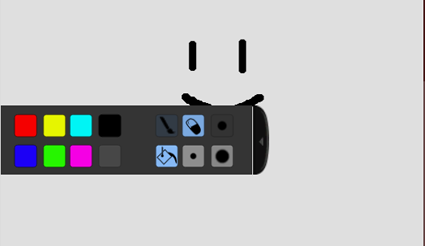
\includegraphics[scale=0.3]{images/Nono/img2.png}}

		\end{frame}	
	
	\begin{frame}{Architecture logicielle} %Découpage de l'application}
		%Archi logi Manutea
		\centerline{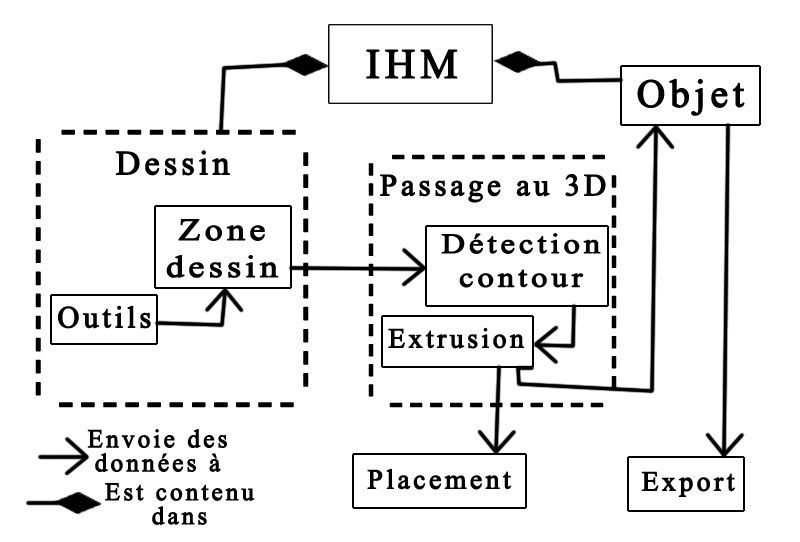
\includegraphics[scale=0.3]{images/archilogi/archi.png}}
		\begin{itemize}
			\item 
		\end{itemize}
	\end{frame}	
	
			
	\section{Etape par étape}
		%Expliquer nos choix par rapports aux objectifs énoncés
	\begin{frame}
		IHM Arnaud
	\end{frame}
	
	\begin{frame}
		Dessin -> Outils Arnaud
	\end{frame}
	
	\begin{frame}
		Dessin -> zone Etienne
	\end{frame}
	
	\begin{frame}
		Aurélien Passage au 3D
	\end{frame}
	
	\begin{frame}
		Placement Arnaud
	\end{frame}
	
	\subsection{Envoi des données}
	
	\begin{frame}{Envoi des données}
		\centerline{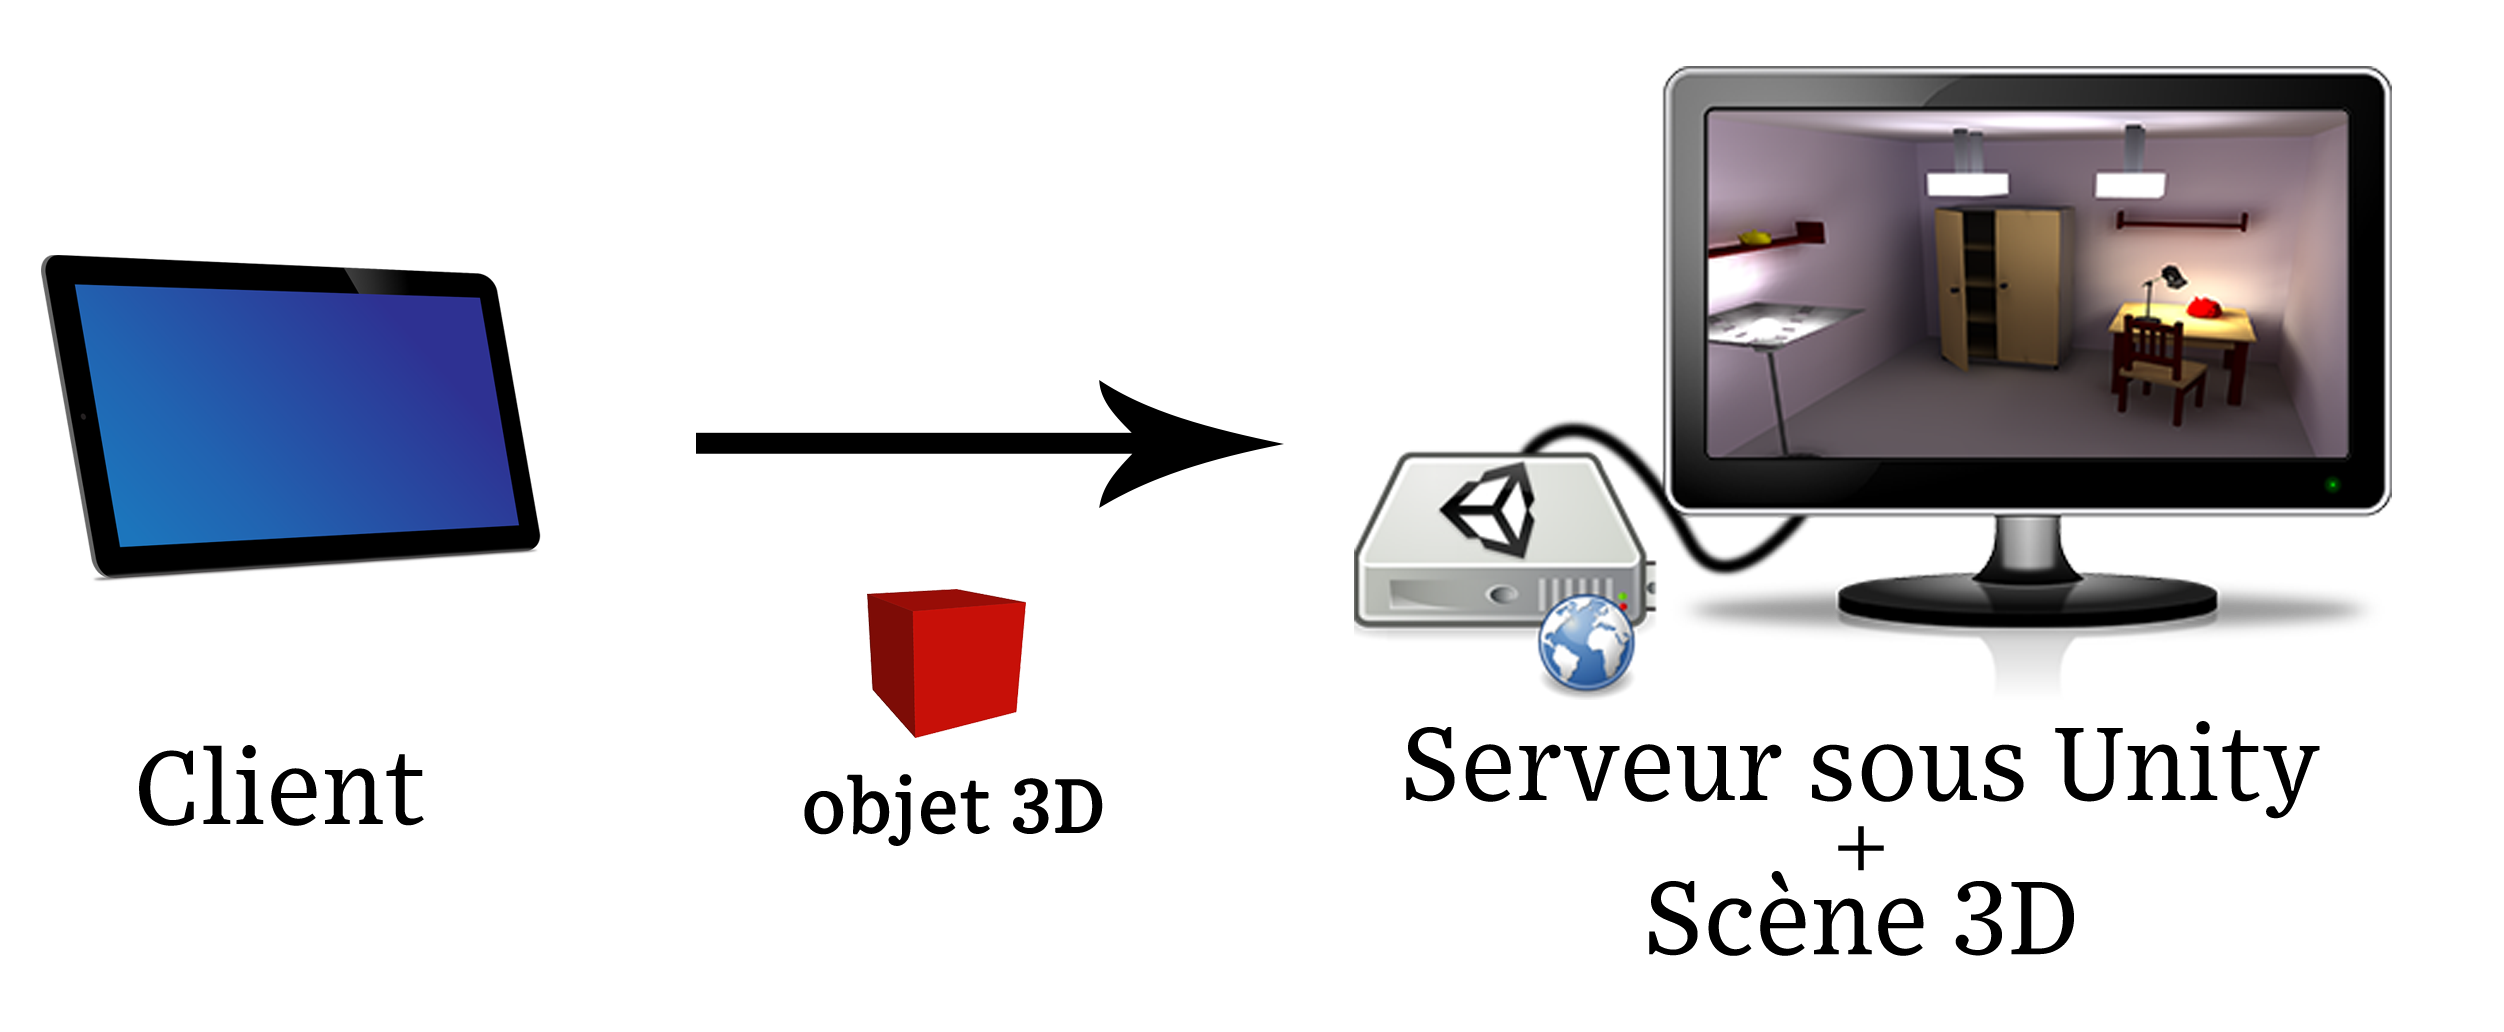
\includegraphics[height=120pt]{images/network/sending_model2.png}}
	\end{frame}
	
	\subsubsection{Côté serveur}
	\begin{frame}{Ajout d'un script}
		\centerline{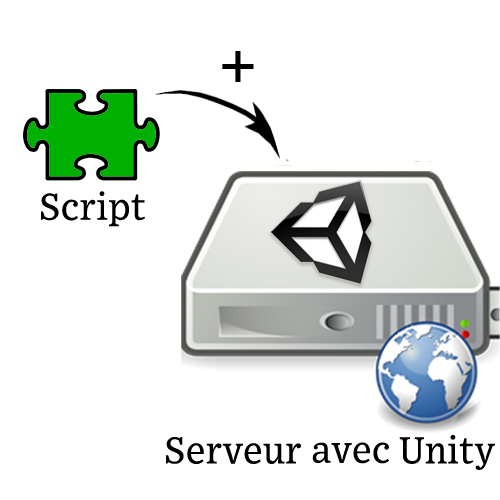
\includegraphics[height=150pt]{images/network/plugin.png}}
		\begin{itemize}	
			\item \pause Léger \pause
			\item Reçoit les données \pause
			\item Intégré dans la scène 3D \pause
			\item Affiche l'objet 
		\end{itemize}	
		
	\end{frame}
	
	\subsubsection{Côté client}
	
	\begin{frame}{Socket TCP}
		\centerline{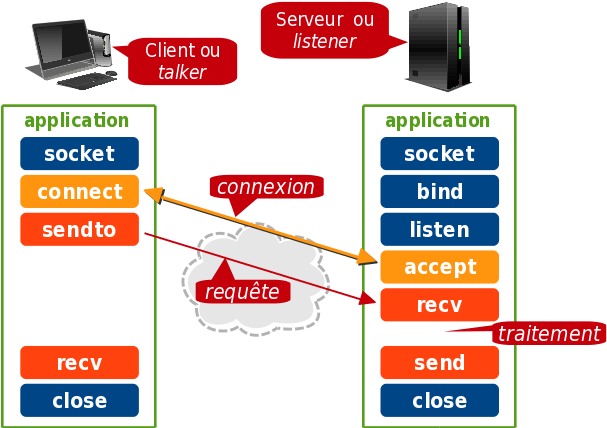
\includegraphics[height=120pt]{images/network/tcp-socket.png}}
		
		\begin{itemize}
			\item Dispose de classes prévues à cet effet en C\#
			\item Documentée en C\# par Microsoft
			\item Permet d'envoyer des octets, donc flexible
		\end{itemize}
	\end{frame}
	
	\begin{frame}{Côté client}
		Export Manutea
	\end{frame}
	
	\section{Conclusion}
	
	\begin{frame}
		Aurélien Conclu
		%vidéo -> présente les points clés de notre présentation
	\end{frame}
		
\end{document}
